% 1. Carregar as bibliotecas necessárias para o TikZ
\usetikzlibrary{positioning, arrows.meta}

% 2. Definir as cores que você usou (exemplos)
\definecolor{steel}{RGB}{70, 130, 180}
\definecolor{soft}{RGB}{240, 240, 240}
\definecolor{accent}{RGB}{0, 150, 0}
\definecolor{crit}{RGB}{200, 0, 0}


\begin{frame}
    \frametitle{Da aplicação do método à crítica}
    \vspace{-0.8em}
    \begin{center}
    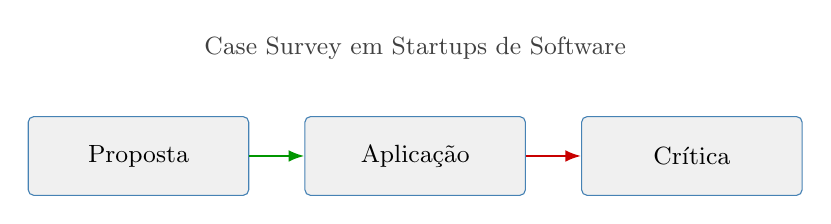
\begin{tikzpicture}[scale=0.9]
        % Nós originais
        \node[draw=steel, rounded corners=2pt, minimum width=2.8cm, minimum height=1cm, fill=soft] (p1) {\small Proposta};
        \node[draw=steel, rounded corners=2pt, minimum width=2.8cm, minimum height=1cm, fill=soft, right=0.7cm of p1] (p2) {\small Aplicação};
        \node[draw=steel, rounded corners=2pt, minimum width=2.8cm, minimum height=1cm, fill=soft, right=0.7cm of p2] (p3) {\small Crítica};
        
        % Novo texto inserido como um nó ancorado acima de 'p2'
        \node[above=0.6cm of p2, text=darkgray, font=\small] {Case Survey em Startups de Software};
        
        % Setas
        \draw[-{Latex[length=2mm]}, thick, accent] (p1) -- (p2);
        \draw[-{Latex[length=2mm]}, thick, crit] (p2) -- (p3);
    \end{tikzpicture}
    \end{center}
\end{frame}